\usetikzlibrary{calc}
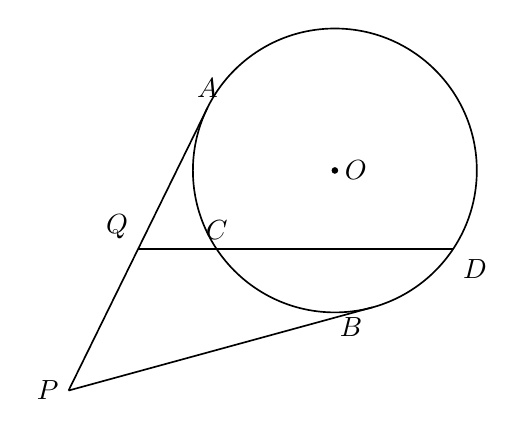
\begin{tikzpicture}[x=1cm,y=1cm,line width=.6pt,font=\normalsize]
\coordinate (O) at (4.8820,3.9950);
\coordinate (P) at (1.5000,1.2000);
\coordinate (Q) at (2.3820,2.9950);
\coordinate (A) at (3.2640,4.7900);
\coordinate (B) at (5.3580,2.2562);
\coordinate (C) at (3.3820,2.9950);
\coordinate (D) at (6.3820,2.9950);
\draw (O) circle[radius=1.8028cm];
\draw (P)--(A);
\draw (P)--(B);
\draw (Q)--(D);
\fill (O) circle[radius=1.2pt];
\node[left] at (P) {$P$};
\node[above left] at (Q) {$Q$};
\node[above] at (A) {$A$};
\node[below left] at (B) {$B$};
\node[above] at (C) {$C$};
\node[below right] at (D) {$D$};
\node[right] at (O) {$O$};
\end{tikzpicture}
